%*****************************************
\chapter{3D Spieleentwicklung mit Java}\label{ch:beispiele}
%*****************************************

\section{Allgemeiner Aufbau von 3D Spielen}\label{sec:aufbau}

Bei 3-dimensionalen Spielen wird das Spielgeschehen in einen Raum transferiert und dem Spieler die Möglichkeit gegeben sich dort frei bewegen zu können. \newline
Im Gegensatz zu 2-dimensionalen Spielen sind hier deutlich mehr Berechnungen auf vektorieller Ebene notwendig, was sich auf die Laufzeit niederschlägt. Daher ist es besonders wichtig ein effizientes Programm zu generieren.
Diesbezüglich ist Java nicht die optimale Programmiersprache, da durch den Interpreter viel Zeit verloren geht. \newline
Dennoch können mit Java sehr schöne und funktionale Spiele erstellt werden.
\\
Im Allgemeinen kann man sagen, dass die meisten 3D Spiele folgende Elemente enthalten:
\begin{itemize}
	\item 3D-Modelle und eine räumliche Spielumgebung
	\item Eine sog. "Kamera", welche nur den relevanten Teil des Bildes abbildet
	\item Möglichkeiten der Interaktion
\end{itemize}



\bigskip

\section{Funktionsweise und Auswahl von Game Engines}\label{sec:jMonkeyEngine}
Um nicht sämtliche mathematischen Berechnungen auf der Grafikkarte selber programmieren, oder beispielsweise die Lautsprecher für Audio-Effekte ansprechen zu müssen, erhält der Entwickler Unterstützung durch sogenannte "Game Engines".
Diese beinhalten die Basisfunktionen von Spielen und ermöglichen dem Spiele-Programmierer eine gezieltere Entwicklung. Zu den Basisfunktionalitäten gehören im Allgemeinen die folgenden \cite{BF1}:
\begin{enumerate}
	\item Grafik-Engine
	\item Physiksystem
	\item Soundsystem
	\item Zustandsspeicherung
	\item Steuerung
	\item Datenverwaltung
\end{enumerate}
Zur Auswahl stehen eine Vielzahl von verschiedenen Engines, welche jeweils vor und Nachteile mit sich bringen. Da wir auf jeden Fall lernen wollten, wie die grundlegenden Dinge funktionieren, haben wir nach Engines gesucht, welche nur die Basisfunktionalitäten unterstützen, jedoch keine automatische Codegenerierung, Drag and Drop oder Editoren beinhalten.
Im folgenden eine Übersicht einiger Engines:


\begin{table}
	\myfloatalign
	\begin{tabularx}{\textwidth}{Xll} \toprule
		\tableheadline{GameEngine} & \tableheadline{Vorteile} & \tableheadline{Nachteile} \\ \midrule 
		Unity & Viele Benutzer, beliebt &  zu oberflächlich, kein Java \\
		jMonkeyEngine & Sehr entwicklungsnahe, Java & Schlechte Dokumentation \\
		Wurfel Engine & Benutzerfreundlich & Keine Physikunterstützung \\
		Cry Engine & Sehr schöne Grafik & Kein Java \\
		\bottomrule
	\end{tabularx}
	\caption[Engines]{Vor - und Nachteile einiger Game Engines \cite{GE1}}  \label{tab:example}
\end{table} 
Letztendlich fiel die Entscheidung auf die jMonkeyEngine, welche häufig von Java Entwicklern verwendet wird. 


\subsection {Die jMonkeyEngine}
Die jMonkeyEngine (jME) ist komplett in Java geschrieben und basiert auf dem Buch "3D Game Engine Design" von David Eberly \cite{GE2}.
Durch eine Abstraktionsschicht kann jedes beliebige Rendering System verwendet werden, beispielsweise die Lightweight Java Game Library (LWJGL) oder die Open Graphics Library (OpenGL).
Die neuste Version ist jME3, welche einige hilfreiche Funktionen mit sich bringt, wie beispielsweise ein Partikelsystem, Frustum Culling oder 3D Sound Unterstützung \cite{JM1}.
\begin{description}
	\item[Frustum Culling:] "Frustum Culling ist eine Optimierungsmethode, bei der all die Objekte vom Zeichnen ausgeschlossen werden, die außerhalb des Sichtbereichs (des Frustums) liegen." \cite{FC1}
\end{description}


\section{Umsetzung in Programmcode}\label{sec:code}
Im folgenden wird beschrieben wie einzelne Elemente in der jMonkeyEngine programmiert werden können und was dabei zu beachten ist. Die Erklärungen orientieren sich hierbei an dem jme3 Online-Beginners-Guide \cite{BG1} und der entsprechenden Dokumentation.

\subsection{Erzeugung der Application-Klasse: SimpleApplication}
Die Main-Klasse jedes jME3 Spieles erbt von der Klasse SimpleApplication, welche ein Spiel darstellt.
In der main-Methode wird dann eine neue Instanz erstellt und anschließend gestartet.

Jede Unterklasse der SimpleApplication beinhaltet die folgenden Methoden:
\begin{enumerate}
	\item simpleInitApp():
	Sorgt für das Laden von Modellen, der Erstellung einer räumlichen Umgebung sowie jegliche Initiierungen.
	\item simpleUpdate(float tpf):
	Wird für jedes frame per second (fps) ausgeführt und kümmert sich um gegebenenfalls geänderte Spielzustände.
	\item simpleRender(RenderManager rm):
	Wird stets nach simpleUpdate aufgerufen und zeichnet das Sichtbild des Spielers neu. Dazu bekommt die Methode einen RenderManager übergeben, welcher Präferenzen beim Zeichnen berücksichtigt (z.B. welche Ebene vorne oder hinten gezeichnet werden soll).
\end{enumerate} Die erste der drei Methoden wird stets zu Beginn ausgeführt um alle benötigten Elemente bereit zu stellen.

\subsection{Funktionsweise von Nodes}
Um Elemente zum Renderingprozess hinzuzufügen, um sie also sichtbar zu machen, müssen diese an ensprechende "Nodes" (engl. Knoten) angehängt werden.
Hierbei gibt es je nach Verwendungszweck verschiedene Arten zum Beispiel die \emph{audioNode} für Soundobjekte oder die \emph{guiNode} für Elemente auf der Benutzeroberfläche.\\
Final werden alle Nodes an die rootNode, also die Wurzel, angehängt. Im  Programmcode funktioniert dies mit der Methode \emph{attachChild()} bzw. \emph{detachChild()} zum entfernen.\\
Selbstverständlich können Objekte auch direkt an die rootNode angehängt werden, weshalb die Methodenparameter Modelle, Nodes, Bilder aber auch beispielsweise Audio-Files sind.
Allerdings ist es empfehlenswert eine geeignete Baumstruktur zu erstellen um so bestimmte Elemente in Gruppen anzusprechen.\\

\colorbox{grau}{\parbox{\dimexpr\textwidth-8\fboxsep}{\centering
\underline{\smash{Beispiel:}} Erzeugung einer eigenen Node durch:
\begin{center}
	\fcolorbox{grau}{white}{Node myNode = new Node();}
\end{center}

Wird nun beispielsweise die folgende Funktion auf dem Konten ausgeführt,
\begin{center}
	\fcolorbox{grau}{white}{myNode.doSomething();}	
\end{center}

so wird diese auch für sämtliche Kinder des Knotens ausgeführt.
}}

\subsection{Modelle und Assets}
Sämtliche externe Gegenstände des Spiels werden im \emph{assets}-Ordner im jME3 Projekt gesammelt. Dies sind multi-media Dateien wie 3D-Modelle, Soundfiles, Texturen, Shader und was sonst noch benötigt wird.
Um diese aus dem Ordner ins Spiel zu laden wird der sogenannte \emph{AssetManager} benötigt, welcher einfach eine Instanz der Klasse mit entsprechenden Funktionalitäten ist. \\Modelle sind dreidimensionale Gebilde welche verschiedenste Elemente in einem Spiel sein können. Hierbei verwendet jME3 die Klasse Spatial (engl. für "räumlich"). \\Zum Laden eines Objektes wird die entsprechende Funktion \emph{loadTexture(String path)} bzw. \emph{loadModel(String path)} aufgerufen und der entsprechende Pfad zum Modell übergeben:
\begin{center}
\fcolorbox{grau}{white}
{Spatial baum = assetManager.loadTexture("Models/Baum.j3o");}
\end{center} Für Modelle gibt es viele verschiedene Datentypen. Neben dem jMonkey-eigenen Dateiformat .j3o existieren einige weitere. Selbstverständlich ist meist eine Konversion zwischen den Formaten möglich. Die häufigsten von uns angetroffenen Vertreter für Modell-Deklarationen sind die folgenden:
\begin{enumerate}
	\item XML-Dateien: Aus einer mesh.xml Datei wird ein Objekt erzeugt. 
	\item OBJ-Dateien: Ein von \emph{Wavefront Technologies} entwickeltes Dateiformat für geometrische Formen. \cite{OBJ1}
	\item Blender-Dateien: Dies sind Dateien aus der Blender-Software, mit welcher Modelle erzeugt werden können.
\end{enumerate} Wie bereits unter \emph{Funktionsweise von Nodes} beschrieben müssen die Spatials nun lediglich zur rootNode, bzw. einer anderen Node welche mit der rootNode verknüpft ist, hinzugefügt werden. Damit werden die Modelle und Texturen sichtbar und sind Teil des Rendering-Prozesses.


\begin{center}
	\fcolorbox{grau}{white}
	{rootNode.attachChild(baum);}
\end{center} Der Aufbau von Modellen erfolgt durch entsprechende Software mit Polygonzügen oder Punktwolken. Dies definiert die allgemeine Struktur von Objekten.\\
Neben dieser und dem Material (vgl. \emph{Materialien}) gibt es noch das Skelett. Dieses kann ebenfalls in einem entsprechenden Programm wie Blender erzeugt und daraus bestimmte Bewegungsabläufe in Spielen bestimmt werden.
Das Skelett ist notwendig für Animationen von Modellen wie beispielsweise Gehen, Springen oder Ähnlichem.\\
In unserem Progman-Spiel haben wir uns für eine First-Person Perspektive entschieden, wodurch keine Animationen für den Spieler notwendig waren. Darüber hinaus haben wir uns auf Grund des Zeitaufwandes gegen eine Implementierung eines Skeletts beim Progman entschieden. Dieser ist daher nur eine starre Figur.



\subsection{Materialien}
Da in Modell-Software vorerst nur die Form von Figuren bestimmt wird, muss anschließend noch die Farbe, die Oberflächenstruktur und das Lichtverhalten bestimmt werden. Dies funktioniert über sogenannte \emph{'materials'}.\\
Die Datei für das Material kann in jme3 mit der Endung .mtl identifiziert werden. Diese bildet die entsprechenden Farbwerte von Bilddateien auf das Modell ab. Als Farbgeber sind beispielsweise mat.jpg oder mat.png gängig. Darüber hinaus können durch eine \emph{bump-map} und \emph{normalen}-Formate die Struktur der Oberfläche sowie das Verhalten bei Lichteinstrahlung (bspw. spiegelnd / schattierend /...) festgelegt werden. \\ Mit diesen Werkzeugen können sehr detaillierte Modellgenerierungen erfolgen, die nahezu realitätsgetreu sind.



\begin{figure}[h!]
	\myfloatalign
	\subfloat[Modell ohne Material]
	{
	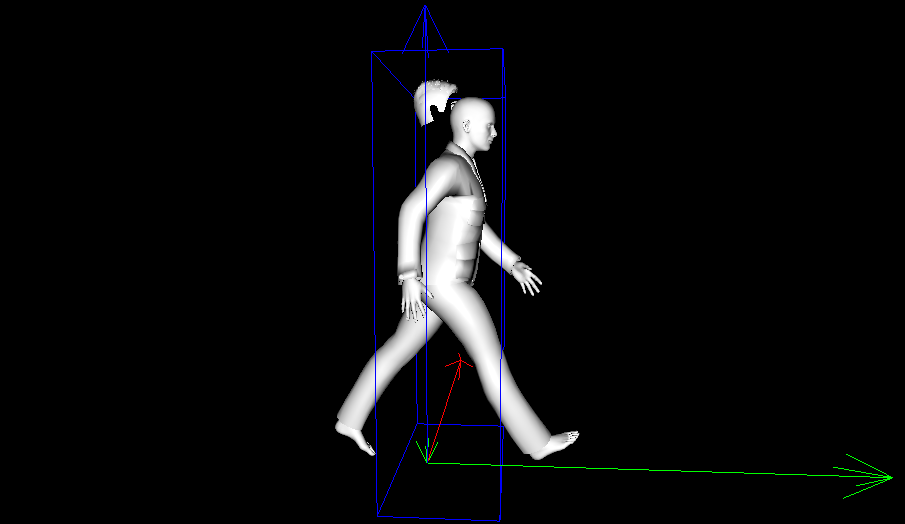
\includegraphics[width=.3\linewidth, height = 70pt]{images/modelmat}} \quad
	\subfloat[Modell mit Material]
	{\label{fig:example-b}%
	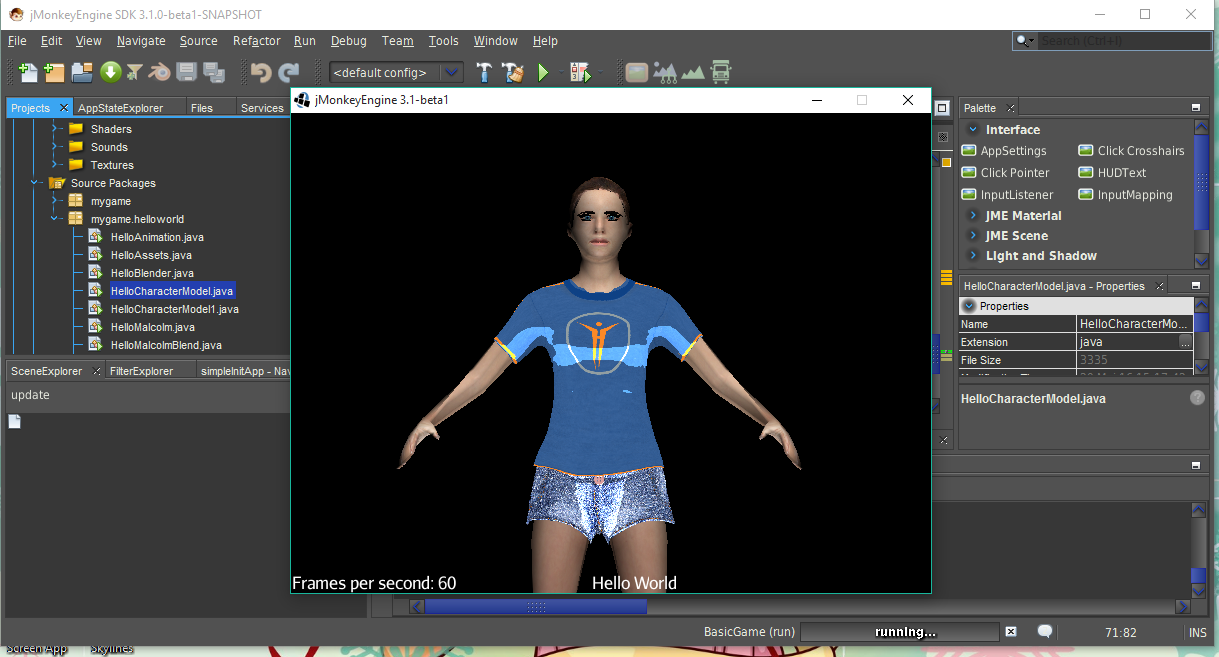
\includegraphics[width=.3\linewidth, height = 70pt]{images/modelmat2}} \\
	\caption[Materials auf Modellen]{Modell mit und ohne Material \cite{Fig1}}\label{fig:example}
	
\end{figure}







\subsection{User-Input}

Aus einem 3-dimensionalen Gebilde wird erst dann ein Spiel, wenn Interaktion mit dem Spieler stattfindet. Dazu müssen Tasteneingaben, Mauseingaben oder gegebenfalls auch Toucheingaben abgefangen und verarbeitet werden.
Hierbei werden die aus der ProkSy-Vorlesung bekannten Listener-Klassen verwendet.
Bezogen auf unser Spiel wurden folgende Aktionen durch Listener abgefangen:
\begin{enumerate}
	\item W/A/S/D: Dient zur Bewegung innerhalb des Spielraumes.
	\item Pfeiltasten/Maus: Zur Rundumsicht entsprechend einer Kopf-Bewegung.
	\item Taste "B": Aufnahme eines gefundenen Buches.
	\item Taste "L": Ein-/Ausschalten der Taschenlampe.
	\item Leertaste: Sprung
\end{enumerate} Zur Realisierung stehen in jme3 zwei wichtige Listener-Klassen zur Verfügung: Der \emph{ActionListener} und der \emph{AnalogListener}.
Ersterer sollte verwendet werden, wenn einzelne Aktionen erfolgen wie z.B. einmaliges Drücken der Taste B, zum Aufsammeln eines Buches.\\
Die zweite Klasse widerum, falls dauerhafte Events wie Gedrückthalten von W zur Vorwärtsbewegung abgefangen werden sollen. \\
Im Programmcode müssen dann entsprechende Aktionen erfolgen, damit der Input auch eine Auswirkung auf das Spiel hat. Beim Drücken von W müsste etwa der Richtungsvektor sowie die aktuelle Position abgefangen werden um eine Vorwärtsbewegung um x = walkingSpeed Richtungseinheiten zu erzeugen.

\subsection{Kollisionserkennung}
Damit man als Charakter nicht durch die gesamte Spielwelt gehen kann, müssen entsprechende Kollisionserkennungen eingebaut werden. So sollte der Spieler beispielsweise stoppen, wenn er sich in einen Baum hinein bewegen würde. Dazu kann in der Engine der folgende Code realisiert werden:


\colorbox{grau}{\parbox{\dimexpr\textwidth-8\fboxsep}{\centering
		\begin{center}
			\fcolorbox{grau}{white}{	CollisionShape shape = CollisionShapeFactor.createMeshShape(treeShape);}
		\end{center}
		\begin{center}
			\fcolorbox{grau}{white}{baumControl = new RigidBodyControl(shape);}	
		\end{center}
		\begin{center}
		\fcolorbox{grau}{white}{baum.addControl(baumControl);}	
		\end{center}
}}\bigskip \\Im ersten Schritt wird eine Form erstellt, welche das Modell annähert oder teilweise sogar mit ihm übereinstimmt. Bei Bäumen reichen theoretisch auch einfache Zylinder, da man mit der Baumkrone im Spiel sowieso nicht in Kontakt kommt. Im obigen Beispiel wird allerdings auf das Mesh, d.h  die tatsächliche Form zurückgegriffen.\\
Danach wir ein Art 'Überwacher' instantiiert, welcher sich um die Kollisionsfunktionalität kümmert. Dieser "kontrolliert" wann sich Modelle überlappen und verhindert dadurch ein Bewegen durch diese. Optional kann als Parameter auch die physikalische Masse des Objekts übergeben werden.\\
Im letzten Schritt wird dieser Control zum gewünschten Objekt hinzugefügt, damit eine entsprechende Kollisionserkennung stattfinden kann.\\
Bei Erzeugung einer Spielumgebung im \emph{SceneComposer} werden die physikalischen Eigenschaften bereits implizit implementiert.


\subsection{Erzeugung einer Spielumgebung}
Terrain oder SceneComposer, sky, 
Funktionalität und allgemeines vorgehen.
Wichtig: Beschreibung von Licht nicht vergessen (sonst dunkel)

\subsection{Hinzufügen von Audio}
Bei großen rollen-basierten Spielen erzeugen die Sound-Effekte, neben den grafischen Eigenschaften, den Hauptbestandteil der entsprechenden Atmosphäre. In unserem Spiel wurden folgende Sound-Effekte verwendet:
\begin{enumerate}
	\item Horror-Theme Soundtrack als Hintergrundmusik
	\item Donner-und Regensounds, welche zufällig abgespielt werden
	\item Fußstapfen im Wald
	\item Spezial Effekte wie beispielsweise: Knisterndes Feuer, Wolfs-Heulen, Spieler-Atmen, Herzklopfen...
\end{enumerate} Um Audio dem Spiel hinzuzufügen sind beispielhaft die folgenden Code-Zeilen notwendig.

\begin{lstlisting}
audio_nature = new AudioNode(assetManager,"Sound/nature.mp3", true);
audio_nature.setLooping(true);  // activate continuous playing
audio_nature.setPositional(true);   
audio_nature.setVolume(3);
rootNode.attachChild(audio_nature);
audio_nature.play();
}
\end{lstlisting}


\subsection{Physikalische Modellierung}
Die jme3 Engine erlaubt durch ihre Physik-Engine Objekten verschiedenes physikalisches Verhalten zuzuordnen. Die Kräfte, welche wirken sind dann je nach Masse verschieden.\\
In unserem Spiel haben wir hauptsächlich von der Schwerkraft Gebrauch gemacht, welche sich durch den Befehl\emph{ setGravity()} auf Spatials anwenden lässt.

\subsection{Effekte und Details}
Um dem Spiel mehr Leben einzuhauchen können verschiedenste Spezialeffekte erstellt werden. Im Folgenden wird auf zwei wichtige Beispiele eingegangen und wie diese in der jMonkeyEngine umgesetzt werden können.
\subsubsection{Nebel}
In unserem Wald haben wir zur besseren Atmosphäre einen Nebeleffekt hinzugefügt. Genaugenommen ist dies lediglich eine Erhellung der Pixel in Abhängigkeit des Abstandes vom Spieler. 
Fog Filter... Entsprechende Berechnung kann in unter \cite{Cr14} nachvollzogen werden.

\[
FinalFogColor = (1.0-e^{db\textrm{1}}*fogColor + e^{db\textrm{1}} * lightColor
\]

\begin{figure}[h!]
	\myfloatalign
	\caption{Exponentieller Nebel - Ergebnis}
	
	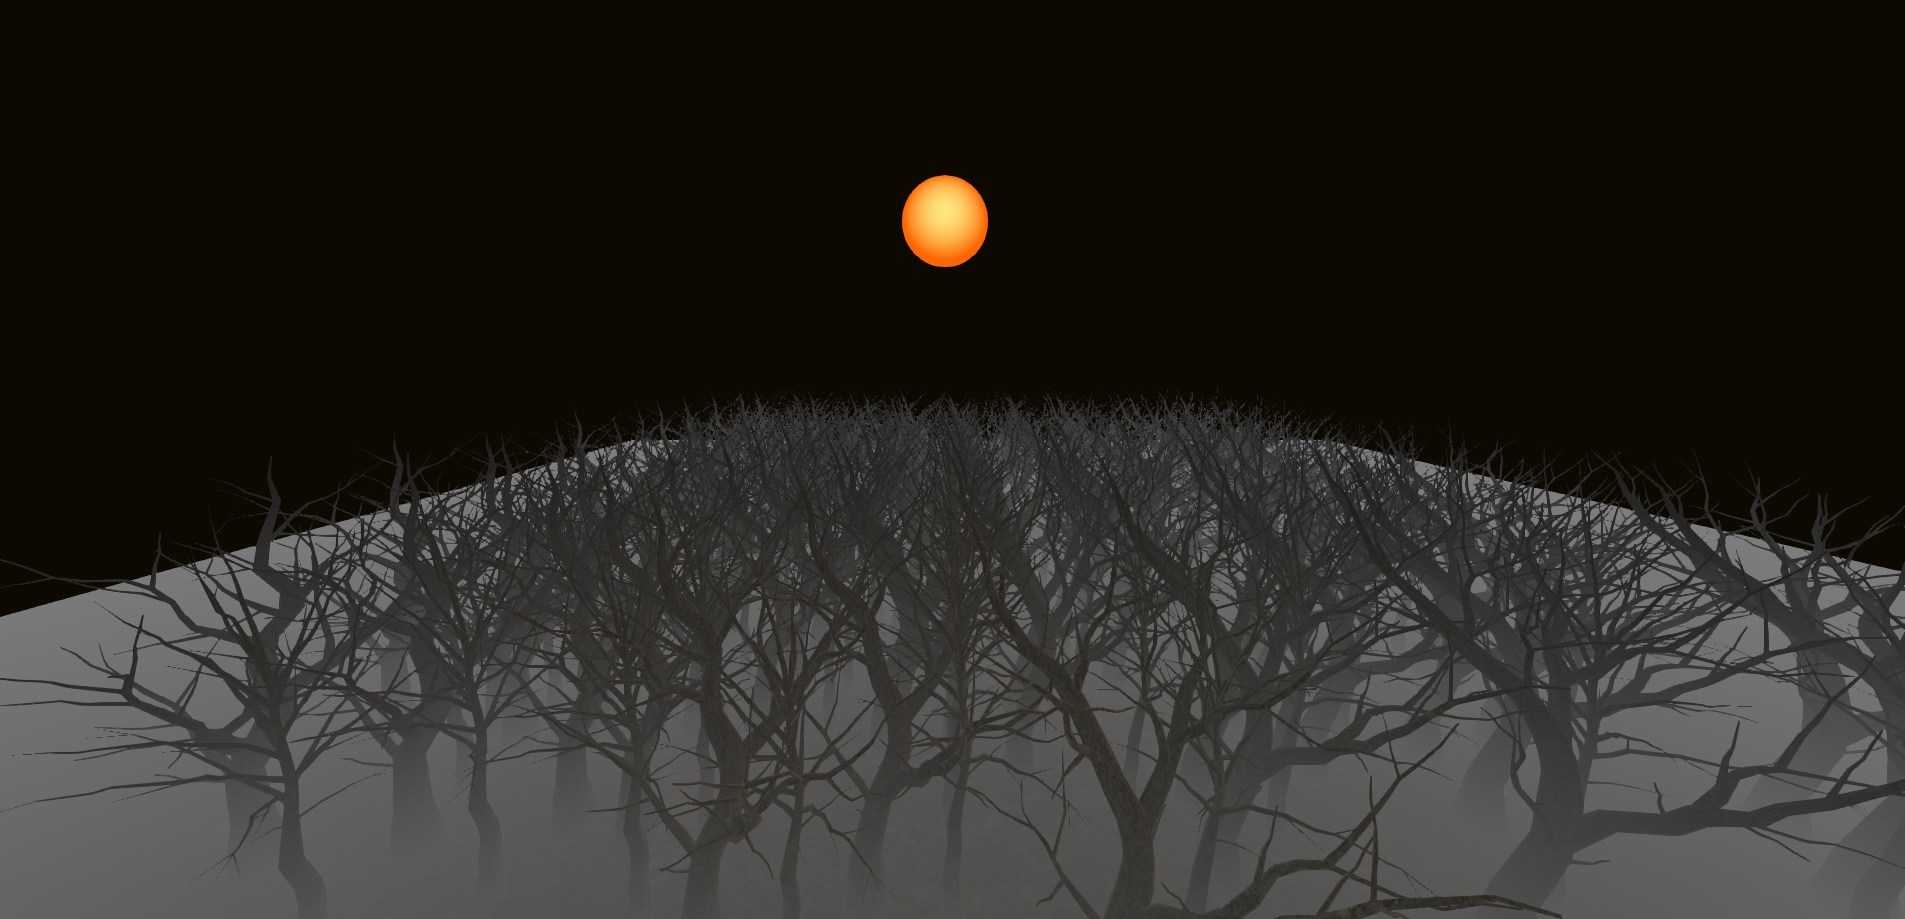
\includegraphics[width=.9\linewidth, height = 200pt]{images/fog} 
	
\end{figure}

\subsubsection{Partikeleffekte}
Feuer, Regen... usw...


\section{Optimierung des Programms}\label{sec:optimizing}
Wenn man wie oben beschrieben einige Modelle und Effekte in seine Spielumgebung einbindet, kann das sehr schnell für ein Laptop zu aufwendig werden, dieses Spiel zu rendern. Dabei spielt die Anzahl der Vertexes bzw. Triangles eine zentrale Rolle. Jedes Modell hat unter Umständen einige tausend Triangles, sodass sich das in einem Spiel sehr leicht addieren kann. In unserem Spiel gibt es zum Beispiel knapp 2000 Bäume, welche alle gerendert werden müssen: Vereinfacht man dort das Modell des Baumes, hat dies viel Potenzial, das gesamte Spiel zu beschleunigen. Mit Hilfe von F5 kann man in jMonkey während des Spiels anzeigen lassen, wie viele Triangles und Vertexes gerade zu rendern sind. Es versteht sich von selbst, dass ein Spiel mit einigen Millionen Vertexes viel zu aufwendig wird zu rendern, weshalb die Framerate auf nahezu 0 sinken kann. Um dies zu verhindern, muss man also die Anzahl an Triangles und Vertexes verringern. Dies ist grundsätzlich durch die Minimierung der Anzahl von Modellen oder durh die Minimierung der Anzahl an Triangles und Vertexes innerhalb eines Modells möglich. Diese haben damit ein sogenanntes LevelOfDetail (kurz LOD). Interessant zu beobachten ist zudem, dass ein Terrain selbst (also der Ground) sehr viele Triangles besitzen kann. Das liegt daran, dass diese Terrains dafür ausgelegt sind, dass sie aufwendige Umgebungen darstellen müssen. So können Gebirge oder sonstige Unebenheiten sehr fein dargestellt werden. Der Nachteil dabei ist jedoch, dass es dadurch sehr aufwendig wird die Texture selbst ohne Models zu rendern, obwohl diese wie in unserem Beispiel einfach nur gerade sein kann. Es ist also unbedingt notwendig bei der Programmierung eines 3D-Spiels auf die Framerate und Komplexität der Welt zu achten.



\subsubsection{Minimierung der Anzahl von Modellen}

\subsubsection{Level of Detail (LOD)}
In der jMonkeyEngine ist es grundsätzlich vorgesehen, dass man seinen Modellen eigene LODs gibt. Damit kann man anhand dieser LODs die Komplexität des Models im Laufe des Spiels bzw. vor dem Spiel verändern. Dabei gilt es noch zu beachten, dass die Modelle selbst keine LODs haben, sondern die Geometrys, welchen sie zugrunde liegene. Man kann innerhalb des SceneExplorers die einzelnen Modelle und deren Geometries auswählen, und eigene LODs generieren:

GRAFIK generateLOD.png

Ein alternativer Weg wäre, dass man der Geometry eines vorhandenen Spatials während der Laufzeit einen neuen LOD zuweist. 



